 \documentclass[tikz,border=0cm]{standalone}
\usepackage{type1cm}
\usepackage{fp}
\usetikzlibrary{decorations.pathmorphing}
\usetikzlibrary{decorations.fractals}
\usetikzlibrary{calc}
\usetikzlibrary{shadows}

\usepackage{fetamont}
%\usepackage[rm,light]{roboto}
%\usepackage[scaled]{helvet}
%\usepackage{avant}
%\renewcommand{\familydefault}{\sfdefault}
\usepackage{cmbright}

\usepackage{bm,amsmath,amssymb}
\usepackage{soul}
\usepackage{minted}
\usepackage{tcolorbox}
\usepackage{wrapfig}
\usepackage{multirow}
\usepackage{graphicx}

\newcommand{\clm}{Cl\'{e}ment }
\newcommand{\norm}[1]{\lVert#1\rVert}

\edef\myfontscale{1.7}

\definecolor{edblue}{RGB}{4, 80, 124}
\definecolor{eyellow}{RGB}{248, 176, 23}
\definecolor{elblue}{RGB}{55, 172, 195}
\definecolor{bg}{rgb}{0.95,0.95,0.95}

%% scalable vector fonts
\edef\fontSizeX{12}\edef\fontSizeY{14}
\FPupn{\resulttinyX}{myfontscale fontSizeX * 2 round}
\FPupn{\resulttinyY}{myfontscale fontSizeY * 2 round}
\renewcommand*{\tiny}{\fontsize{\resulttinyX}{\resulttinyY}\selectfont}

\edef\fontSizeX{14.4}\edef\fontSizeY{18}   
\FPupn{\resultscriptsizeX}{myfontscale fontSizeX * 2 round}
\FPupn{\resultscriptsizeY}{myfontscale fontSizeY * 2 round}
\renewcommand*{\scriptsize}{\fontsize{\resultscriptsizeX}{\resultscriptsizeY}\selectfont}

\edef\fontSizeX{17.28}\edef\fontSizeY{22}
\FPupn{\resultfootnotesizeX}{myfontscale fontSizeX * 2 round}
\FPupn{\resultfootnotesizeY}{myfontscale fontSizeY * 2 round}
\renewcommand*{\footnotesize}{\fontsize{\resultfootnotesizeX}{\resultfootnotesizeY}\selectfont}

\edef\fontSizeX{20.74}\edef\fontSizeY{25}
\FPupn{\resultsmallX}{myfontscale fontSizeX * 2 round}
\FPupn{\resultsmallY}{myfontscale fontSizeY * 2 round}
\renewcommand*{\small}{\fontsize{\resultsmallX}{\resultsmallY}\selectfont}

\edef\fontSizeX{24.88}\edef\fontSizeY{30}
\FPupn{\resultnormalsizeX}{myfontscale fontSizeX * 2 round}
\FPupn{\resultnormalsizeY}{myfontscale fontSizeY * 2 round}
\renewcommand*{\normalsize}{\fontsize{\resultnormalsizeX}{\resultnormalsizeY}\selectfont}

\edef\fontSizeX{29.86}\edef\fontSizeY{37}
\FPupn{\resultlargeX}{myfontscale fontSizeX * 2 round}
\FPupn{\resultlargeY}{myfontscale fontSizeY * 2 round}
\renewcommand*{\large}{\fontsize{\resultlargeX}{\resultlargeY}\selectfont}

\edef\fontSizeX{35.83}\edef\fontSizeY{45}
\FPupn{\resultLargeX}{myfontscale fontSizeX * 2 round}
\FPupn{\resultLargeY}{myfontscale fontSizeY * 2 round}
\renewcommand*{\Large}{\fontsize{\resultLargeX}{\resultLargeY}\selectfont}

\edef\fontSizeX{43}\edef\fontSizeY{54}
\FPupn{\resultLARGEX}{myfontscale fontSizeX * 2 round}
\FPupn{\resultLARGEY}{myfontscale fontSizeY * 2 round}
\renewcommand*{\LARGE}{\fontsize{\resultLARGEX}{\resultLARGEY}\selectfont}

\edef\fontSizeX{51.6}\edef\fontSizeY{64}
\FPupn{\resulthugeX}{myfontscale fontSizeX * 2 round}
\FPupn{\resulthugeY}{myfontscale fontSizeY * 2 round}
\renewcommand*{\huge}{\fontsize{\resulthugeX}{\resulthugeY}\selectfont}

\edef\fontSizeX{61.92}\edef\fontSizeY{77}
\FPupn{\resultHugeX}{myfontscale fontSizeX * 2 round}
\FPupn{\resultHugeY}{myfontscale fontSizeY * 2 round}
\renewcommand*{\Huge}{\fontsize{\resultHugeX}{\resultHugeY}\selectfont}

\edef\fontSizeX{74.3}\edef\fontSizeY{93}
\FPupn{\resultveryHugeX}{myfontscale fontSizeX * 2 round}
\FPupn{\resultveryHugeY}{myfontscale fontSizeY * 2 round}
\newcommand*{\veryHuge}{\fontsize{\resultveryHugeX}{\resultveryHugeY}\selectfont}

\edef\fontSizeX{89.16}\edef\fontSizeY{112}
\FPupn{\resultVeryHugeX}{myfontscale fontSizeX * 2 round}
\FPupn{\resultVeryHugeY}{myfontscale fontSizeY * 2 round}
\newcommand*{\VeryHuge}{\fontsize{\resultVeryHugeX}{\resultVeryHugeY}\selectfont}

\edef\fontSizeX{107}\edef\fontSizeY{134}
\FPupn{\resultVERYHugeX}{myfontscale fontSizeX * 2 round}
\FPupn{\resultVERYHugeY}{myfontscale fontSizeY * 2 round}
\newcommand*{\VERYHuge}{\fontsize{\resultVERYHugeX}{\resultVERYHugeY}\selectfont}

% set the normalfont (default)
\renewcommand*{\normalfont}{\normalsize}

\usepackage{booktabs,dcolumn}
\usepackage{array}
\newcolumntype{T}{>{\begingroup\bfseries}r<{\endgroup}}
\newcolumntype{N}{D{.}{.}{-1}}
\newcolumntype{R}{D{.}{.}{2.4}}
\newcolumntype{K}{D{.}{.}{3.4}}
\newcommand{\imgcase}[2]{\includegraphics[width=0.5\linewidth]{#1_#2_base}%
\includegraphics[width=0.5\linewidth]{#1_#2_side}}
\usepackage[tableposition=top,font=footnotesize,labelfont=bf,sf]{caption}

\usepackage[margin=1in, paperwidth=48in, paperheight=48in]{geometry}

\begin{document}

\begin{tikzpicture}[x=70cm, y=100cm]
\fill[white, use as bounding box] (0, 0) rectangle (1, 1);

%%%%%%%%%%%%%%%%%%%%%%%%%%
% Title
%%%%%%%%%%%%%%%%%%%%%%%%%%
\begingroup
\node[inner sep=1cm, 
      fill=eyellow,
      anchor=north, 
      draw=elblue, line width=3.5mm]
      (title)
      at ($(current bounding box.north)$)
  {\begin{minipage}{0.88\textwidth}
   \begin{center}
   {\ffmfamily\bfseries\color{black}
   {\LARGE fenicstools} \\[0.4ex]
   {\LARGE smart add-ons for FEniCS}}

   \bigskip
   {\color{edblue}
     \textbf{M.~Mortensen and M.~Kuchta}

   \vskip-5mm\footnotesize
   \texttt{mikaem@math.uio.no and mirok@math.uio.no}}

   \end{center}
  \end{minipage}};

  \node[anchor=west] (foo) at ($(current bounding box.north west)+(7cm, -4.6cm)$)
  {
    
\includegraphics[height=7cm]{graphics/fenicslogo}
  };
  \node[anchor=east] (foo) at ($(current bounding box.north east)+(-7cm, -4.6cm)$)
  {
    
\includegraphics[height=7cm]{graphics/qrfenicstools}
  };
\endgroup

%%%%%%%%%%%%%%%%%%%%%%%%%%%%%%%%%
% Introduction, no frame
%%%%%%%%%%%%%%%%%%%%%%%%%%%%%%%%%
\node[anchor=north]
(motif title)
at ($(current bounding box.north)+(0cm,-9.5cm)$)
{
\begin{minipage}{0.6\textwidth}
\centering
{
  fenicstools is a collection of extensions to the FEniCS library with 
  particular focus on efficient visualization and postprocessing of large 
  scale computations.
}
\end{minipage}
};

%%%%%%%%%%%%%%%%%%%%%%%%%%%%%%%%%
% Clement
%%%%%%%%%%%%%%%%%%%%%%%%%%%%%%%%%
\node[draw=elblue, 
      fill=eyellow!20!white,
      line width=1mm, anchor=north west,
      rounded corners=4mm, inner sep=1cm,
      minimum height=20cm]
(clm)
at ( $(current bounding box.north west) + (1cm, -15cm)$ )
{\begin{minipage}{40cm}   % 70 cm take 40
\vspace{0.5cm}
\footnotesize
  Evaluating quantities derived from primary unknowns, e.g. strain from
  displacement, is a frequent part of computational loops. Such quantities often
  lack the $H^2$ regularity required for nodal interpolation and therefore can
  be computed in FEniCS only by $L^2$ projection. An alternative method is the 
  \clm interpolation - a numerical technique for constructing interpolants of
  $H^1$ functions based on local regularization.
%

\vspace{1cm}
\begin{minipage}{0.58\textwidth}
\textbf{$\triangleright$ Figure}:
{fenicstools implements the lowest order \clm interpolation operator resulting
  in a CG$_1$ approximation of interpolated function $f$. The degree of freedom 
  at $x_j$ is computed as $v$ minimizing $\norm{f-v}^2_{0, {w}_j}$ over
  constant fields on patch $w_j$. The interpolation error is controlled on 
  the union $\tilde{w}_K$. Therefore no power $h$ is lost in the error estimates:
  \[
    \norm{u - I_h u}_{m, K} \leq C h^{1-m}_K\norm{u}_{1, \tilde{w}_K}
  \]
  for $u\in H^1$, $m=0, 1$ and $K$ an element of triangulation.
}
\end{minipage}
\hfill
\begin{minipage}{0.4\textwidth}
\begin{center}
\includegraphics[width=0.8\textwidth]{./graphics/domains}
\end{center}
\end{minipage}

\vspace{1cm}
\begin{minipage}{0.4\textwidth}
\begin{center}
\includegraphics[width=\textwidth]{./graphics/plot_Ih}\\
\includegraphics[width=\textwidth]{./graphics/plot_Ih_clement}
\end{center}
\end{minipage}
\hfill
\begin{minipage}{0.58\textwidth}
\textbf{$\triangleleft$ Figure}:{
  The local regularization procedure results in smearing of gradients. 
  However, the largest errors are localized near the boundaries where the
  interpolant(bottom figure) fails to preserve the boundary values.
}\\
  \textbf{$\triangledown$ Figure}:{fenicstools supports \clm interpolation of 
  all\textsuperscript{*} valid UFL expressions. How about evaluating 
  $\boldsymbol{w}=\nabla\cdot(\boldsymbol{u}\otimes\nabla v)$
  for $\boldsymbol{u}\in\left[\text{CG}_1\right]^2$, $v\in\text{CG}_1$ or 
  $\boldsymbol{w}=\sin(\det\nabla \boldsymbol{u})$ where $\boldsymbol{u}$ is a 
  vector field in $\mathbb{R}^3$?\\
  \vspace{0.5cm}
  \begin{center}
  \includegraphics[height=12cm]{./graphics/rate_plot}
  \end{center}
}
\end{minipage}

% % Implementation
%   Unlike $L^2$ projection, which requires solution of large linear system, \clm 
%   interpolant is constructed from local linear systems of size 1 assembled over
%   patches surrounding mesh vertices. In fenicstools this mapping is realized
%   more efficiently using a precomputed averaging operator $A$ such that 
%   $Ab(u)=I_h u$. Due to this choice the setup cost of the interpolant is higher
%   (4x) than that of $L^2$ projector. However, the subsequent (repetitive)
%   evaluation comes at a cost of a matrix-vector product.
% 
% \vspace{1cm}
% \begin{center}
% \begin{tabular}{l|ccccc}
% \hline
% \multirow{2}{*}{$n$} & \multicolumn{5}{c}{size}\\
% \cline{2-6}
%    &       132098 &   526338     &      2101250 &       8396802 &      14612418\\
% \hline
% %1  & (0.05, 0.28) & (0.23, 1.19) & (0.95, 5.04) & (4.20, 20.93) & (7.34, 39.79)\\
% %2  & (0.02, 0.18) & (0.08, 0.79) & (0.33, 3.08) & (1.11, 15.48) & (2.16, 27.95)\\
% %4  & (0.00, 0.12) & (0.02, 0.44) & (0.06, 1.73) & (0.28, 6.86)  & (0.80, 15.45)\\
% %8  & (0.00, 0.09) & (0.02, 0.40) & (0.02, 1.31) & (0.17, 4.78)  & (0.21, 11.36)\\
% %16 & (0.00, 0.06) & (0.00, 0.25) & (0.01, 0.88) & (0.04, 3.60)  & (0.09, 7.36) \\
% 1  & (0.07, 0.32) & (0.23, 1.21) & (0.99, 5.17) & (4.10, 20.93) & (7.46, 37.21)\\
% 2  & (0.03, 0.19) & (0.12, 0.76) & (0.66, 3.49) & (2.74, 14.04) & (3.95, 26.42)\\
% 4  & (0.04, 0.20) & (0.09, 0.45) & (0.68, 2.21) & (1.49, 10.80) & (2.03, 19.06)\\
% 8  & (0.02, 0.09) & (0.09, 0.43) & (0.33, 1.61) & (0.76, 8.46) & (1.82, 13.89)\\
% 16 & (0.02, 0.07) & (0.04, 0.32) & (0.18, 1.06) & (0.72, 7.46) & (1.65, 13.36)\\
% \hline
% \end{tabular}
% \end{center}

Unlike $L^2$ projection, which requires solution of large linear system, \clm 
interpolant is constructed from local linear systems of size 1 assembled over
patches surrounding mesh vertices.

\begin{wraptable}{r}{0.42\textwidth}
\begin{flushright}
\begin{tabular}{c|ccc}
\hline
\multirow{2}{*}{CPUs} & \multicolumn{3}{c}{degrees of freedom}\\
\cline{2-4}
   &       2101250 &       8396802 &      14612418\\
\hline
1  &  (1.0, 5.2) & (4.1, 21.0) & (7.5, 37.2)\\
2  &  (0.7, 3.5) & (2.7, 14.0) & (4.0, 26.4)\\
4  &  (0.7, 2.2) & (1.5, 10.8) & (2.0, 19.1)\\
8  &  (0.3, 1.6) & (0.7,  8.5) & (1.8, 13.9)\\
16 &  (0.2, 1.1) & (0.7,  7.5) & (1.7, 13.4)\\
\hline
\end{tabular}
\end{flushright}
\end{wraptable} 
%------------------------------------------
In fenicstools the mapping is realized more efficiently using a precomputed 
averaging operator $A$ such that $Ab(u)=I_h u$. Due to this choice the setup cost
of the interpolant is higher (4x) than that of $L^2$ projector. However, the 
subsequent (repetitive) evaluation comes at a cost of a matrix-vector product.
\textbf{$\triangleright$ Table}: MPI.MAX-ed timings (in seconds) of action of 
\clm interpolator and $L^2$ projector. 
%
\footnotesize
\end{minipage}};
% 
\node[anchor=west, rounded corners=3mm, fill=eyellow]
(clm title)
at ($ (clm.north west)+(4cm, 0cm) $)
{
  \ffmfamily\textcolor{edblue}{\clm interpolation}
};

%%%%%%%%%%%%%%%%%%%%%%%%%%%%%
% Probes and Structured grids
%%%%%%%%%%%%%%%%%%%%%%%%%%%%%
\node[draw=elblue, 
      fill=eyellow!20!white,
      line width=1mm, anchor=north east,
      rounded corners=4mm, inner sep=1cm,
      minimum height=38cm, minimum width=25cm]
(grid)
at ( $(current bounding box.north east) + (-1cm, -15cm)$ )
{\begin{minipage}{22cm}   % 70 cm take 40
\vspace{0.5cm}
\footnotesize
A turbulent flow simulation often requires setting a probe at a certain 
location inside the flow, where regular samplings are made over time. This can 
  be done efficiently with \emph{Probes} and \emph{StatisticsProbes} classes. 
\vspace{1.0cm}
%\begin{minipage}{\textwidth}
\footnotesize
\begin{tcolorbox}
\begin{minted}{python}
from dolfin import *
from numpy import array
from fenicstools import Probes
mesh = UnitSquareMesh(10, 10)
V = FunctionSpace(mesh, "CG", 1)
x = array([[0.1, 0.1], [0.5, 0.5]])
probes = Probes(x.flatten(), V)
u = project(Expression("x[0]*x[1]"), V)
probes(u)   # evaluate probes once
print probes.array() # [ 0.01  0.25]
\end{minted}
\end{tcolorbox}
\textbf{$\vartriangle$ Code}: Probe two locations defined by the \emph{x} array.
%\end{minipage}

\vspace{1.0cm}
\begin{minipage}{0.58\textwidth}
\textbf{$\triangleright$ Figure}:{
The \emph{StructuredGrid} class allows you to set probes in a 2$d$ slice 
through a 3$d$ (or 2$d$) geometry - or it can be used to set probes in a 3$d$ box for 
some interesting part of the simulated geometry. The slice may be stored as VTK 
  file and viewed, e.g., in Paraview.}
\end{minipage}
\hfill
\begin{minipage}{0.4\textwidth}
\begin{center}
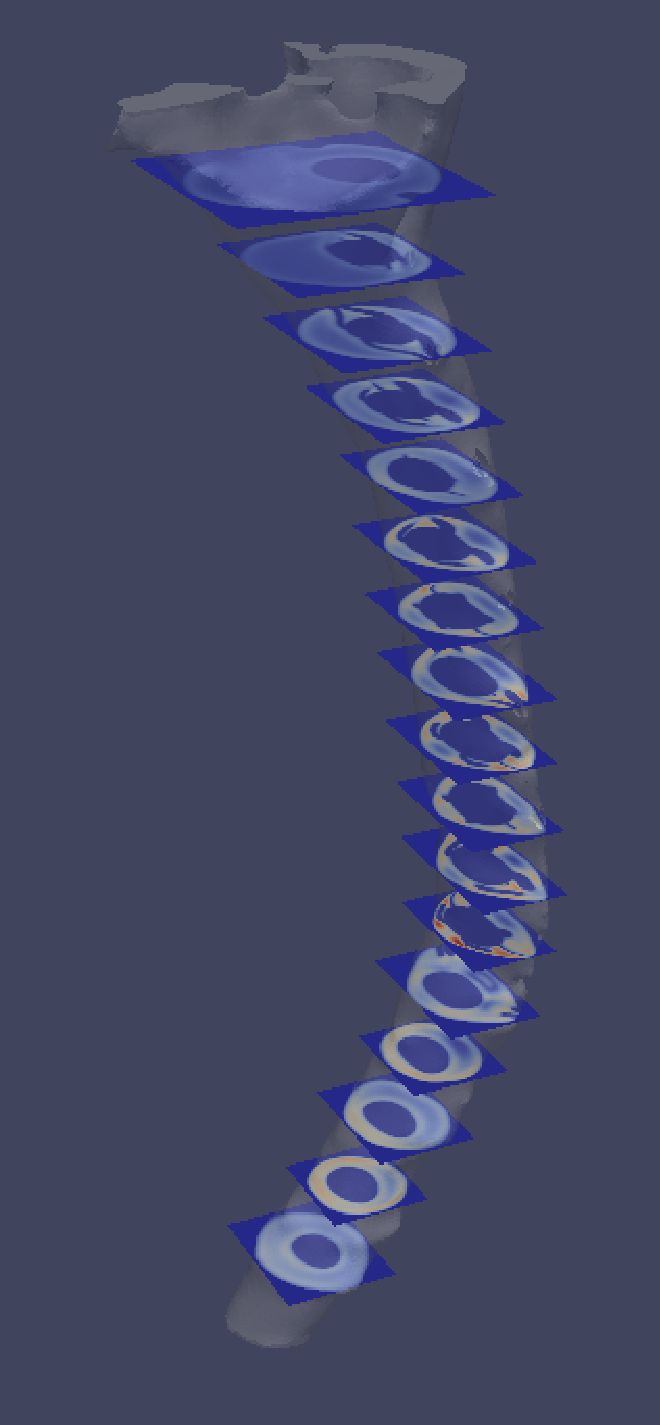
\includegraphics[height=14cm]{./graphics/csf_sliced2.pdf}
\end{center}
\end{minipage}

\footnotesize
\end{minipage}};
% 
\node[anchor=west, rounded corners=3mm, fill=eyellow]
(grid title)
at ($ (grid.north west)+(4cm, 0cm) $)
{
  \ffmfamily\textcolor{edblue}{Probes \& Structured grids}
};
 
%%%%%%%%%%%%%%%%%%%%%%%%%%%%%
% Lagrangian particles
%%%%%%%%%%%%%%%%%%%%%%%%%%%%%
\node[draw=elblue, 
      fill=eyellow!20!white,
      line width=1mm, anchor=north,
      rounded corners=4mm, inner sep=1cm,
      minimum height=39.5cm, minimum width=25cm]
(lp)
at ( $(grid.south)+(0cm, -2cm)$ )
{\begin{minipage}{22cm}   % 70 cm take 40
\vspace{0.5cm}
\footnotesize
  Transport problems $C_t+\boldsymbol{u}\cdot\nabla C=0$ with dominant convection
  can often become more numerically tractable by employing the Lagrangian description 
  of flow. The field $C$ then remains constant in time along the characteristics
  \[
    \boldsymbol{x}_t = \boldsymbol{u}(\boldsymbol{x}, t)
  \]
  and the problem reduces to computing the curves tangent to the velocity field 
  $\boldsymbol{u}$. In fenicstools the Lagrangian tracking is implemented via
  \emph{LagrangianParticles} class. 

\vspace{1cm}
%\begin{minipage}{\textwidth}
\footnotesize
\begin{tcolorbox}
\begin{minted}{python}
lp = fenicstools.LagrangianParticles(V)
x0, C0 = rand((10, 2)), rand(10)
lp.add_particles(x0, {C: C0})
lp.step(u, dt=dt)  # Time integration
\end{minted}
\end{tcolorbox}
\textbf{$\vartriangle$ Code}: Single step of the transport problem.
%\end{minipage} 
 
\vspace{1cm}
\begin{minipage}{0.48\textwidth}
  \textbf{$\triangledown \triangleright$ Figure:} {\emph{LagrangianParticles} were 
  successfully used to study drug delivery and mixing in a cerebrospinal fluid 
  flow.
}
\vspace{0.3cm}
\begin{center}
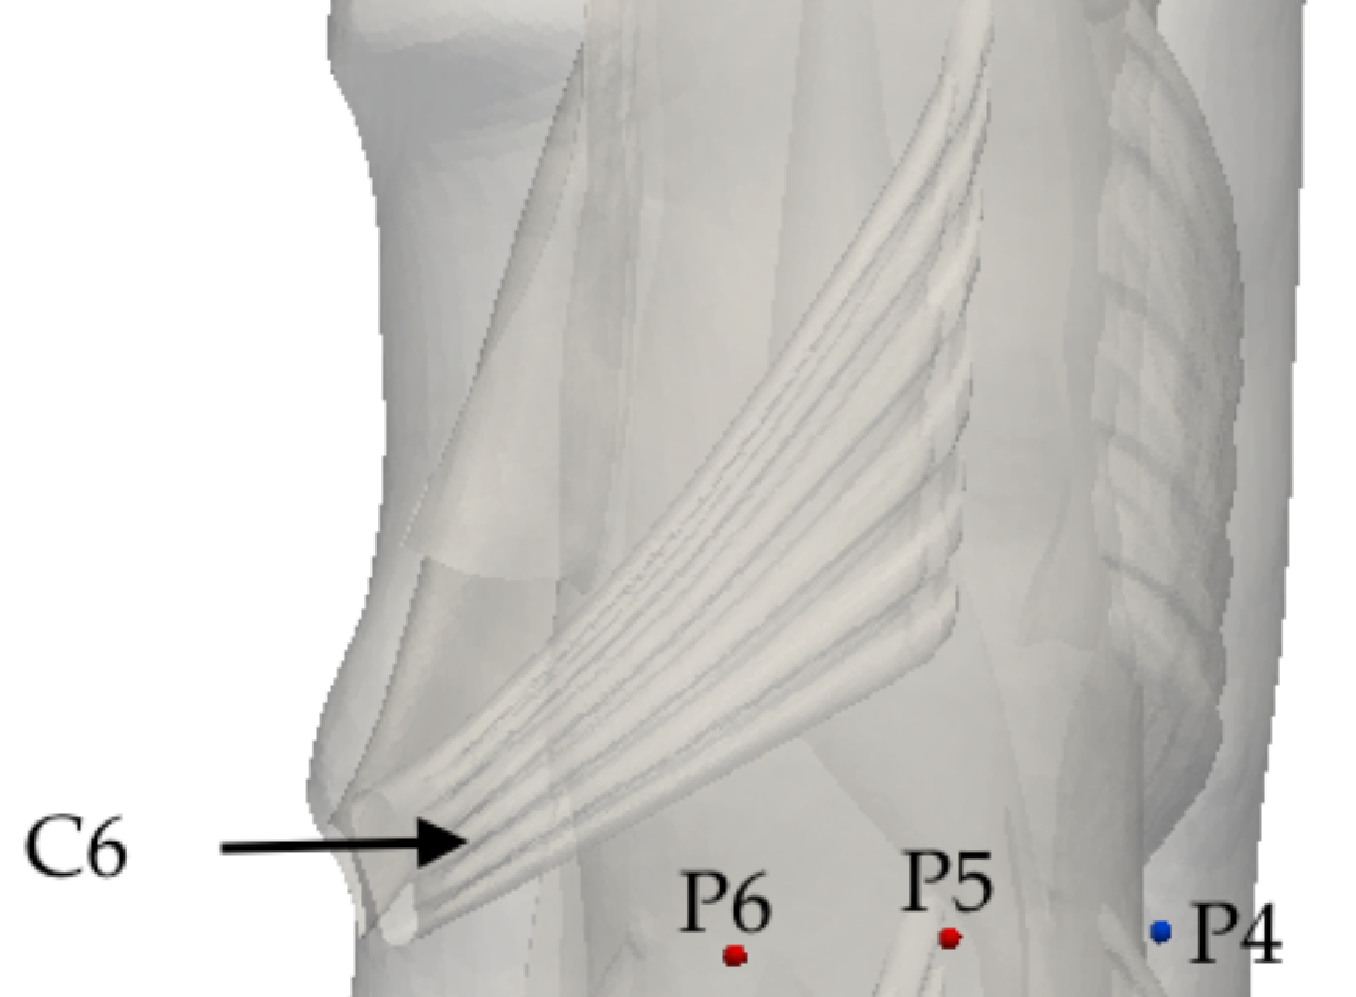
\includegraphics[width=\textwidth]{graphics/position}
\end{center}
\end{minipage}
%
\hfill
%
\begin{minipage}{0.48\textwidth}
\begin{center}
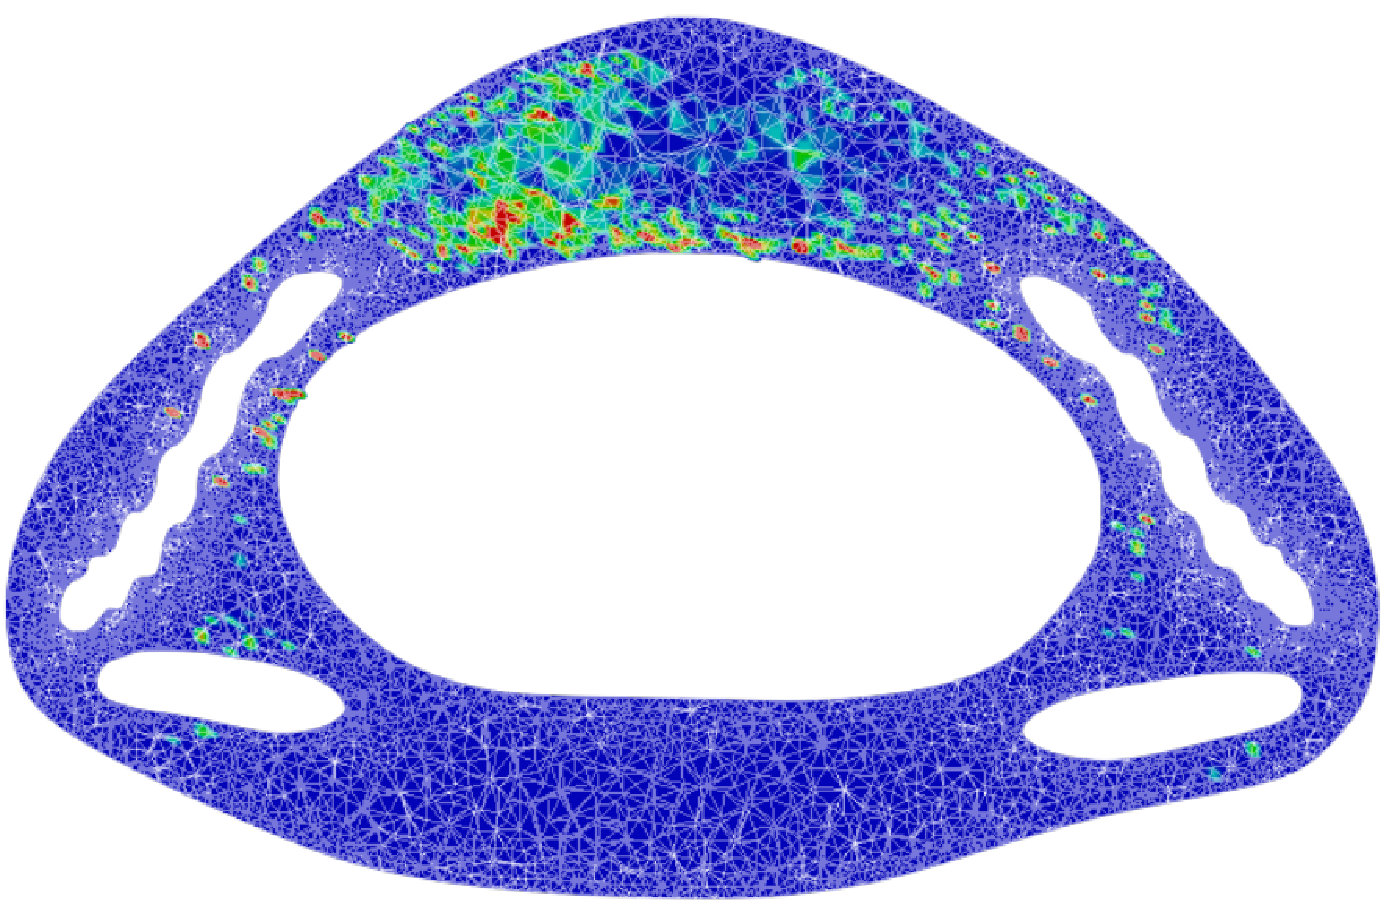
\includegraphics[width=\textwidth]{graphics/p4}\\
\vspace{0.5cm}
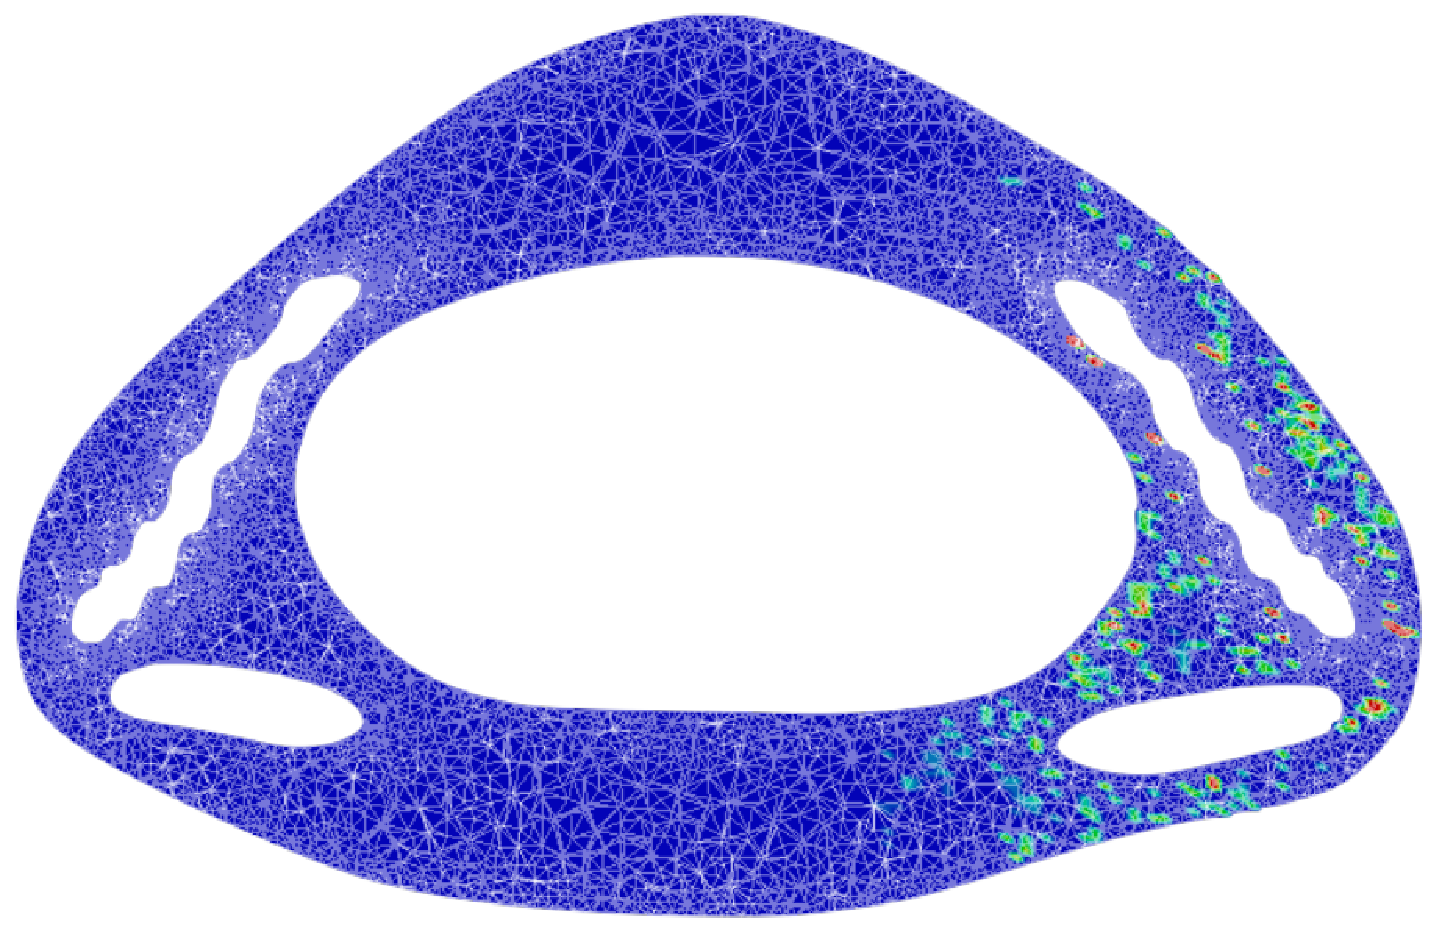
\includegraphics[width=\textwidth]{graphics/p5}
\end{center}
\end{minipage}

\footnotesize
\end{minipage}};
% 
\node[anchor=west, rounded corners=3mm, fill=eyellow]
(lp title)
at ($ (lp.north west)+(4cm, 0cm) $)
{
  \ffmfamily\textcolor{edblue}{Lagrangian tracking}
};

%%%%%%%%%%%%%%%%%%%%%%%%%%%%%
% Travis integration
%%%%%%%%%%%%%%%%%%%%%%%%%%%%%
\node[draw=elblue, 
      fill=eyellow!20!white,
      line width=1mm, anchor=north,
      rounded corners=4mm, inner sep=1cm,
      minimum height=15.25cm, minimum width=42cm]
(travis)
at ( $(clm.south)+(0cm, -2cm)$ )
{\begin{minipage}{40cm}   % 70 cm take 40
\vspace{0.5cm}
\footnotesize
%
\begin{minipage}{0.66\textwidth}
fenicstools is developed using Travis Continuous Integration and Anaconda 
Cloud. With Travis CI all tests are automatically executed in an Ubuntu environment 
on travis-ci.org for each new commit or pull request to origin/master. A tailored 
Anaconda build of a recent FEniCS version is then used in a MiniConda environment 
and tests start within minutes. 

\vspace{1cm}
\begin{tcolorbox}
\begin{minted}{python}
conda config --add channels mikaem/label/travis
conda config --add channels mikaem
conda install fenics=1.7.0 pyvtk h5py=2.6.0
\end{minted}
\end{tcolorbox}
\textbf{$\vartriangle$ Code}: Setting up FEniCS with conda.
\end{minipage}
\hfill
\begin{minipage}{0.33\textwidth}
%\begin{figure}
\begin{center}
  {
\includegraphics[height=6cm]{./graphics/travislogo}}\\
  \vspace{1cm}
  {
\includegraphics[height=6cm]{./graphics/anacondalogo}}
\end{center}
%\end{figure}
%
\end{minipage}
%
\footnotesize
\end{minipage}};
% 
\node[anchor=west, rounded corners=3mm, fill=eyellow]
(travis title)
at ($ (travis.north west)+(4cm, 0cm) $)
{
  \ffmfamily\textcolor{edblue}{Development cycle}
};

%%%%%%%%%%%%%%%%%%%%%%%%%%%%%
% Footer
%%%%%%%%%%%%%%%%%%%%%%%%%%%%%
\begingroup
\draw[fill=eyellow, draw=none] { 
  ($(current bounding box.south west)+(0cm, 43.5mm)$) --
  ($(current bounding box.south east)+(0cm, 43.5mm)$) -- 
  (current bounding box.south east) --
  (current bounding box.south west) -- 
  cycle
};
   %
\draw[elblue, line width=3.5mm]{
  ($(current bounding box.south east)-(0cm, -1.75mm)$) --
  ($(current bounding box.south west)-(0cm, -1.75mm)$)
};
   %
 \draw[elblue, line width=3.5mm]{
   ($(current bounding box.south east)-(0cm, -41.75mm)$) --
   ($(current bounding box.south west)-(0cm, -41.75mm)$)
 };
 \node[anchor=west]
 at ( $(current bounding box.south west)+(1cm, 21.75mm)$ )
 {
\includegraphics[height=4cm,trim=0 0 370 0,clip]{graphics/uiologo}};
    %
\node[anchor=east]
at ( $(current bounding box.south east)+(-1cm, 26.75mm)$ )
{
    
\includegraphics[height=3.0cm,trim=0 0 0 0, clip]{graphics/cbclogo}
};
  % QR Code for poster
\node[anchor=center] (qr1) at ($(current bounding box.south)+(-4cm, 21.75mm)$ ){
    \includegraphics[height=36.5mm]{graphics/qrposter}
};
\node[anchor=east]  at ($(qr1.west)+(0.75cm, 0.0cm)$)
{\footnotesize{\textbf{$\triangleright$}Poster}};

  % QR Code for extras
\node[anchor=center] (qr2) at ($(current bounding box.south)+(+4cm, 21.75mm)$ ){
    \includegraphics[height=36.5mm]{graphics/qrextras}
};
\node[anchor=west]  at ($(qr2.east)+(-0.75cm, -0.0cm)$) 
{\footnotesize{\textbf{$\triangleleft$}Extras}};

\endgroup
\end{tikzpicture}

\end{document}
